\documentclass[10pt,mathserif]{beamer}
\usepackage[english]{babel}
\usepackage[utf8]{inputenc}
\usepackage[T1]{fontenc}
\usepackage{helvet}
\usepackage{nimbusmononarrow}
\usepackage{euler}
\usepackage{tikz}
\usepackage{listings}
\usepackage{relsize}
\usepackage{booktabs}

\usetikzlibrary{arrows}
\usetikzlibrary{backgrounds}
\usetikzlibrary{chains}
\usetikzlibrary{fit}
\usetikzlibrary{positioning}
\usetikzlibrary{scopes}
\usetikzlibrary{trees}
\usetikzlibrary{automata}
\usetikzlibrary{positioning}
\usetikzlibrary{shapes.multipart}

\usetheme{boxes}
%\useoutertheme{essential}
\usecolortheme{seagull}
\usefonttheme{structurebold}
\setbeamertemplate{navigation symbols}{}
\setbeamertemplate{frametitle}
{
	\begin{centering}
		\vspace{1.5em}
		\LARGE
    \insertframetitle
    \par
    \vspace{0.5em}
  \end{centering}
}
\setbeamerfont{title}{size=\huge}
\setbeamerfont{subtitle}{size=\Large}

\lstset{basicstyle=\ttfamily\scriptsize}
\newcommand{\cinput}[1]{\lstinputlisting[language=C,basicstyle=\ttfamily]{#1}}
\newcommand{\cinline}[1]{\lstinline[language=C,basicstyle=\ttfamily]!#1!}
\newcommand{\cppinput}[1]{\lstinputlisting[language=C++,basicstyle=\ttfamily]{#1}}
\newcommand{\cppinline}[1]{\lstinline[language=C++,basicstyle=\ttfamily]!#1!}
\newcommand{\llvminput}[1]{\lstinputlisting[language=LLVM,basicstyle=\ttfamily]{#1}}
\newcommand{\llvminline}[1]{\lstinline[language=LLVM,basicstyle=\ttfamily]!#1!}
\lstdefinelanguage{LLVM}%
  {morekeywords={define,declare,global,constant,internal,external,private,%
      linkonce,linkonce_odr,weak,weak_odr,appending,common,extern_weak,%
      thread_local,dllimport,dllexport,hidden,protected,default,except,deplibs,%
      volatile,fastcc,coldcc,cc,ccc,x86_stdcallcc,x86_fastcallcc,ptx_kernel,%
      ptx_device,signext,zeroext,inreg,sret,nounwind,noreturn,nocapture,byval,%
      nest,readnone,readonly,noalias,uwtable,inlinehint,noinline,alwaysinline,%
      optsize,ssp,sspreq,noredzone,noimplicitfloat,naked,alignstack,module,asm,%
      align,tail,to,addrspace,section,alias,sideeffect,c,gc,target,datalayout,%
      triple,blockaddress},%
  morekeywords=[2]{add,fadd,sub,fsub,mul,fmul,sdiv,udiv,fdiv,srem,urem,frem,%
     and,or,xor,icmp,fcmp,eq,ne,ugt,uge,ult,ule,sgt,sge,slt,sle,oeq,ogt,oge,%
     olt,ole,one,ord,ueq,ugt,uge,ult,ule,une,uno,nuw,nsw,exact,inbounds,phi,%
     call,select,shl,lshr,ashr,va_arg,trunc,zext,sext,fptrunc,fpext,fptoui,%
     fptosi,uitofp,sitofp,ptrtoint,inttoptr,bitcast,ret,br,indirectbr,switch,%
     invoke,unwind,unreachable,malloc,alloca,free,load,store,getelementptr,%
     extractelement,insertelement,shufflevector,extractvalue,insertvalue},%
  sensitive=t,%
  morestring=[b]",%
  morecomment=[l];%
  }[keywords,comments,strings]


\author{Stefano Cherubin}
\institute{Politecnico di Milano}
\date{03-05-2019}
\title{Introduction to LLVM compiler framework}
\subtitle{Course outline}
\newcommand{\customdata}{Stefano Cherubin <stefano.cherubin@polimi.it>}

\AtBeginSection[]
{
\begin{frame}{Contents}
\tableofcontents[currentsection]
\end{frame}
}


\begin{document}

\begin{frame}
\maketitle
\begin{center}
\itshape\scriptsize Welcome slides
\end{center}
\end{frame}

\begin{frame}[plain]{}
  \begin{center}
    \vspace{-.1\textheight}
    
\includegraphics[width=\textwidth]{img/00/logo.png}
  \end{center}
\end{frame}
%--- Next Frame ---%

\begin{frame}[t]{About the dragon}
  \begin{itemize}
    \item The \textbf{LLVM logo} \cite{LOCAL:www/LLVMlogo} is a stylized
          wyvern (a kind of dragon).
          Dragons have connotations of power, speed and intelligence,
          and can also be sleek, elegant, and modular (err, maybe not).
    \pause
    \item There is a series of \textbf{compiler books} dating back to the 1970s
          showing illustrations with dragons and knights
          \cite{Aho:1977:PCD:1095594}
          \cite{Aho:1986:CPT:6448}
          \cite{Aho:2006:CPT:1177220}
  \end{itemize}
  \begin{center}
    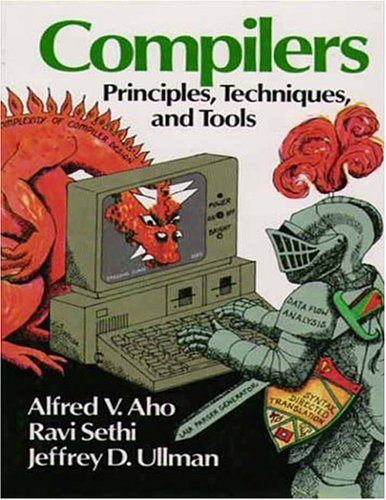
\includegraphics[width=.25\textwidth]{img/00/red_dragon_book.jpg}
    \hfill
    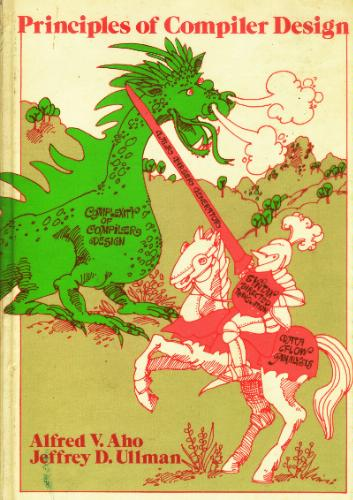
\includegraphics[width=.25\textwidth]{img/00/green_dragon_book.jpg}
    \hfill
    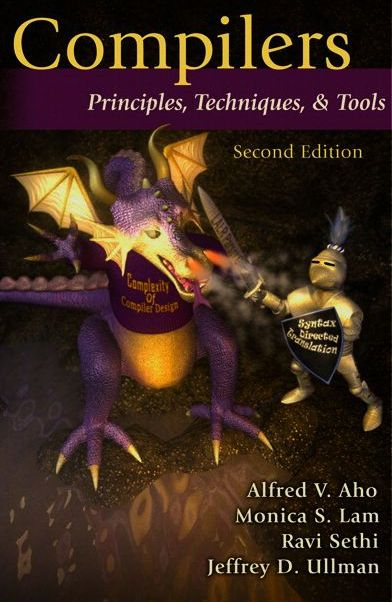
\includegraphics[width=.25\textwidth]{img/00/purple_dragon_book.jpg}
  \end{center}
\end{frame}
%--- Next Frame ---%

\begin{frame}[t]{About me}
  \begin{huge}
    \texttt{Stefano Cherubin}
  \end{huge}
  \begin{itemize}
    \item \texttt{stefano.cherubin@polimi.it}
    \item PhD candidate @ Politecnico di Milano (Italy)
    \item working on compilers since not so long time
    \item definitly not an experienced knight...
    \pause
    \item ...I'm more like a lazy Hobbit
  \end{itemize}
  \begin{center}
    
\includegraphics[height=.35\textheight]{img/00/lazy_hobbit.jpg}
    \hspace{.1\textwidth}
    
\includegraphics[height=.35\textheight]{img/00/lazy_hobbit_2.jpg}
  \end{center}
\end{frame}
%--- Next Frame ---%

\begin{frame}[t]{About you}
  In order to fully understand the content of this course you should have:
  \begin{itemize}
    \vfill
    \item knowledge of what a compiler is
    \vfill
    \item proficiency in most common data structures
    \vfill
    \item proficiency in Object-Oriented Programming
    \vfill
    \item at least some experience with C++
  \end{itemize}
\end{frame}
%--- Next Frame ---%

\begin{frame}[t]{About the course}
  \begin{Large}
  \vfill
  \begin{enumerate}
    \item First part
      \begin{itemize}
        \vfill
        \item Compiler design
        \vfill
        \item LLVM structure overview
        \vfill
        \item LLVM-IR language
    \end{itemize}
    \vfill
    \item Second part
      \begin{itemize}
        \item LLVM Documentation
        \vfill
        \item Available middle-end passes (overview)
        \vfill
        \begin{itemize}
          \item Normalization
        \vfill
          \item Analysis
        \end{itemize}
        \vfill
        \item LLVM quick start tutorial (depending on time)
      \end{itemize}
  \end{enumerate}
  \vfill
\end{Large}
\end{frame}
%--- Next Frame ---%

\begin{frame}[t]{Goal of the course}
  At the end of these lectures you should:
  \begin{itemize}
    \vfill
    \item understand the LLVM compiler infrastructure
    \vfill
    \item be able to read a .ll file (LLVM-IR)
    \vfill
    \item know where to look for documentation
    \vfill
    \item know which are the main middle-end weapons
          LLVM provides you out of the box
    \vfill
    \item know how to implement a simple analysis / transformation
    \vfill
    \item know how to test your code
  \end{itemize}
\end{frame}
%--- Next Frame ---%

\section*{Bibliography}
\begin{frame}[allowframebreaks]{Bibliography}
\nocite{*}
\bibliographystyle{unsrt}
\bibliography{bibliography-0}
\end{frame}

\end{document}
